\documentclass[11pt]{article}
\usepackage{graphicx}
%\usepackage{mathtools}
\usepackage{amssymb,amsmath}
\usepackage{textcomp}
\DeclareMathOperator*{\argmin}{arg\,min}

%\usepackage{subcaption}
%\usepackage{float}
\usepackage{setspace}
\usepackage{fullpage}
\usepackage[font=scriptsize]{caption}
%\usepackage{fullpage}
%\setcounter{secnumdepth}{1}
\begin{document}

\title{GRN inference in multiple species}
\author{Kari Y. Lam, Zachary M. Westrick, Frank Underwood}
\maketitle

\begin{abstract}
HELLOOOOOOOOOOOOOOOOOOOOOOOO
\end{abstract}

\section{Introduction}

\begin{figure}
\begin{center}
  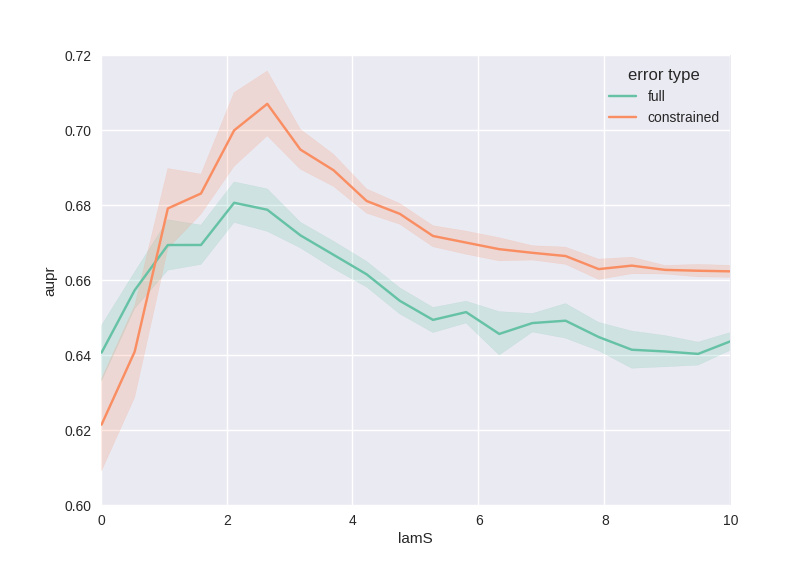
\includegraphics[scale=0.45]{simulated.png}
  \caption{\label{fig:figure1} This is what a figure looks like}
  \end{center}
\end{figure}

\section{Methods}
\subsection{GRN}
We begin with an existing framework for estimating the interaction weights in a gene regulatory network (GRN). In the Inferelator algorithm, linear differential equations are used to model changes in gene expression. The rate at which the expression of gene $i$, $x_i$, changes is governed by degradation of existing transcripts with rate $\alpha$ plus a linear combination of transcription factor (TF) expressions.
\begin{equation}
\frac{\mathrm d}{\mathrm d t} x_i = -\alpha_{i}x_{i} + \sum \beta_{i,j}x_{j}
\end{equation}
We are interested in learning $\beta$, the matrix defining the influence of each TF on each gene. We fix the decay rate $\alpha$ for all genes, and set it assuming a time-constant of 10 minutes [CITATIONS], as in [CITATIONS]. Let $x_i(t)$ be the expression of gene $i$ at time $t$. Given time-series data on the expression of gene $i$ at timepoints $t_k$ and $t_{k+1}$, we can approximate the rate of change of $x_i$ as $x_i'(t_k)=\frac{x_i(t_{k+1})-x_i(t_k)}{t_{k+1}-t_k}$. This gives us, for each gene $i$ and time $t_{k}$ an equation

\begin{equation}
\frac{x_i(t_{k+1})-x_i(t_k)}{t_{k+1}-t_k} + \alpha_{i}x_{i}(t_k)= \sum \beta_{i,j}x_{j}(t_k)
\end{equation}
\noindent We can summarize these equations in matrix form as
\begin{equation}
Y = \beta X
\end{equation}
\noindent We approach the learning of the $\beta$ matrix using regression. Because there are typically far fewer conditions than possible regressors (TFs), we introduce a ridge regularization constraint with weight $\lambda_R$ and solve
\begin{equation}
\argmin_\beta\vert \vert X\beta - Y_2 \vert \vert ^2 + \lambda_R \vert \vert \beta \vert \vert ^2
\end{equation}
This is essentially the same basic formulation as was used in the Inferelator algorithm, which we extend to the case of simultaneously inferring the GRNs of multiple species. 

\subsection{Fused GRN}
We expect related species to be governed by similar but not necessarily identical gene regulatory networks. We approach the problem of cross-species GRN inference by introducing constraints into the above regression formulation to penalize differences between interaction weights that are expected to be similar based on gene orthology. We can then solve the penalized regression problems simultaneously, in order to obtain a GRN for each species. Consider the case of organisms $A$ and $B$, governed by GRNs $\beta^A$ and $\beta^B$ (the following approach applies equally well to more than two species but for simplicity we continue with the case of two species). If TF $g^A$ in organism $A$ and TF $h^B$ in organism $B$ are orthologs, and gene $k^A$ and $l^B$ are orthologs, then we expect that the $g^A \rightarrow k^A$ interaction weight should be similar to the $h^B \rightarrow l^B$ interaction weight, and we introduce a fusion constraint between these analogous interactions. In terms of the above regression formulation, we expect that $\beta^A_{g,k} \approx \beta^B_{h,l}$, and include a penalty term $\lambda_S(\beta^A_{g,k} - \beta^B_{h,l})^2$ to the quantity being minimized in order to ensure similarity. The parameter $\lambda_S$ controls how highly to penalize differences between fused coefficients. This gives us the final equation to be minimized 
\begin{equation}
\argmin_{(\beta^A, \beta^B)} \displaystyle\sum_{S \in (A, B)} \vert \vert X^S\beta^S - Y^S \vert \vert ^2 + \lambda_R \vert \vert \beta^S \vert \vert ^2 + \displaystyle \sum_{\beta^{S_1}_{g,k} \approx \beta^{S_2}_{h,l}} \lambda_S(\beta^{S_1}_{g,k} - \beta^{S_2}_{h,l})^2
\end{equation}
Where the second sum is over pairs of interactions with fusion constraints. Note that each term in the quantity being minimized is an L2 norm of a linear combination of gene expressions, so the entire problem can be solved through linear regression with a suitable design matrix [DETAILS SHOULD GO SOMEWHERE ELSE, OR NOWHERE]. The $\beta$ vectors corresponding to a pair of genes can be solved independently as long as the pair is not linked by fusion constraints, or a chain of fusion constraints; thus the problem of cross-species GRN inference decomposes into a large number of manageable regression problems as long as the orthology mappings are sparse.

[DIGRESSION?]

When there is a one-to-one orthology between the species being considered (ie different cell-lines of the same organism), the choice of $\lambda_S$ allows one to interpolate between fitting each network independently ($\lambda_S=0$) and pooling data together as if it came from one source ($\lambda_S=\inf$). Part of the appeal of the approach, however, is that it allows pooling of data even when there is incomplete orthology. By introducing constraints on the similarity of individual interactions, rather than on the networks as a whole [CITE IBM?], we can pool some information across species even when an arbitrarily small fraction of genes have orthologs. This is particularly useful when dealing with a large number of species; pairwise orthologies may be nearly complete even when the number of genes present in every organism is small. 
\subsubsection{Equivalent prior}
I want to talk about the fusion constraints as a Gaussian prior, and talk about the adjustment stuff

\subsection{Alternative penalty functions}
Sometimes gene orthology is not a good predictor of functional similarity. To simultaneously learn when a gene's function has diverged from that of its ortholog, and improve model selection, we consider alternative penalized least squares approaches. Our fusion penalty pulls beta values for analogous interactions towards each other; since we use an L2 penalty, interaction weights which differ from each other the most are excessively penalized. SCAD [Fan Li 2001] and MCP [Zhang] are two alternative penalties which diminish this bias. Fan and Li point out that the bias can be removed by choosing a constant penalty beyond some threshold. This is analogous to 'unfusing' certain interactions, and easing up on the demand that certain beta values be close in value when doing so strongly opposes minimizing the mean squared error component of the penalty function. SCAD and MCP both use an L1 penalty near the origin, setting small estimated coefficients to zero and choosing a sparse solution. Because we do not expect most fused beta values to be identical, but rather similar, we amend the alternative fusion penalty to be L2 near the origin, resulting in:
\begin{equation}
p_{\lambda,\gamma}(\theta) = \left\{
    \begin{array}{lr}
    \lambda\theta^2-{ \theta^2 \over 2\gamma} & \text{if } \theta \leq \gamma\lambda\\
    {1 \over 2}\gamma\lambda^2 & \text{if } \theta > \gamma\lambda
    \end{array}
    \right. 
\end{equation}
It is more intuitive to think about the derivative of the penalty:
\begin{equation}
p'_{\lambda,\gamma}(\theta) = \left\{
    \begin{array}{lr}
    2\lambda\theta - {\theta \over \gamma} & \text{if } \theta \leq \gamma\lambda\\
    0 & \text{if } \theta > \gamma\lambda
    \end{array}
    \right.
\end{equation}
    

The MCP-like penalty begins by applying the same rate of penalization as the L2, but continuously relaxes the penalization until the rate drops to 0 and the penalty saturates. 
As in [Fan Li], we use local quadratic approximation and solve by iteratively computing ridge regression. 

\subsection{Simulated data}
Generation of simulated data begins with the production of random orthology mappings. We produce a one-to-one orthology by pairing random genes until a specified fraction have been assigned orthologs. This process is carried out separately for TFs and non-TF genes, so that TFs and non-TF genes are never assigned to be orthologous. We then produce a pair of random networks ($B^1$ and $B^2$) as follows. For each unfilled entry in $B^1$ or $B^2$, we enumerate the set $C$ consisting of the entry along with every entry in either matrix to which it is fused. With probability equal to the sparsity rate we assign every entry in $C$ to be 0, otherwise we sample a value $v \sim \mathcal{N}(0,1)$ and independently assign each entry in $C$ to $v + \mathcal{N}(0, \sigma_f^2)$. $\sigma_f$ is a parameter that controls the distribution of differences in the values of fused coefficients, so that the nonzero coefficients of $B^1, B^2$ are distributed as $\mathcal{N}(0, 1 + \sigma_f^2)$.

Given a network $B$, we generate $N$ samples of gene expressions at each of two timepoints. The condition by gene expression matrix for timepoint one, $Y_{T1}$, is sampled randomly from a multivariate Gaussian distribution with identity covariance matrix. $X_{T1}$ is the TF expression sub-matrix of $Y_{T1}$, and consists of columns of $Y_{T1}$ that correspond to TFs. Treating the decay rate as 0, the gene expression matrix at timepoint two, $Y_{T2}$ is sampled as $Y_{T2} = Y_{T1} + BX_{T1}$. This process is carried out separately for each network. 

Following generation of simulated data, we may introduce error into the orthology mapping. This can take the form of discarding a specified fraction of true orthologies (governed by a false-negative rate), or by introducing random false orthologies (governed by a false-positive rate). For convenience, the false-positive rate is specified in units of the number of true orthologs, and not the number of possible orthologs. 

For the purposes of evaluating simulated network recovery, we define a gold standard network as the support of the beta matrices. Priors used in network inference are interactions from the gold standard. The list of priors can be be manipulated to include false positives and false negatives as with the generation of orthologs. 

\subsection{Bacterial data}
We 

is good
Look an equation array
\begin{equation}
\begin{array}{l}
R_i^{\mathrm{input}}(\theta) = c g_i^{\mathrm{input}}\exp(-(\theta - \theta_i)^2 / (2\sigma^2_{\mathrm{input}}))
\\
R_i^{\mathrm{output}}(\theta) = g_i^{\mathrm{output}}\sum_{j=0}^N R_j^{\mathrm{input}}(\theta) \exp(-(\theta_i - \theta_j)^2/(2\sigma^2_{\mathrm{output}})) .
\end{array}
\end{equation}
\bibliographystyle{plain}
\bibliography{paper}

\end{document}

>>>>>>> 34faf0e6aea8fc5a3af9cb49bfcff0b2e3eaa7ed
